\chapter{Solution proposal \& implementation details}\label{chp:solutionProposal}

\epigraph{Do or do not, there is no try.}{Master Yoda}

We have seen that \acrshort{ads} testing is \textit{complex} and that it is difficult to get a good
test coverage (\Cref{sec:adsTestingComplexity}). Furthermore, we have seen that \acrshortpl{llm}
have \textit{emergent abilities} (\Cref{sec:emergentAbilities}). We therefore propose a tool for
\begin{inparaenum}
    \item running a base \acrshort{ads} test case,
    \item enhancing the test case using \acrshortpl{llm},
    \item running the enhanced test case, and
    \item comparing the results of the two runs.
\end{inparaenum}

This will allow us to learn the extent to which \acrshortpl{llm} can be applied for enhancing
\acrlong{ads} test cases. We will survey several \acrshortpl{llm} and evaluate their applicability
for the problem at hand, in light of what we know about \acrshortpl{llm} (\Nref{sec:llmJungle}). We
want to have a pipeline that is able to process several test cases in succession, in order to get a
substantial dataset.

Let the pipeline tool be known as \hefe.~%\info{This name is naturally just a placeholder.}.
The tool follows a natural pipeline structure. We have some base test cases that
need to be ran in order to get a baseline for the results, we then have to
improve these, and run the improved versions and compare them to their original
versions. The architecture of the tool is visualised in \Cref{fig:hefeArch}.

\begin{figure}[h]
    \centering
    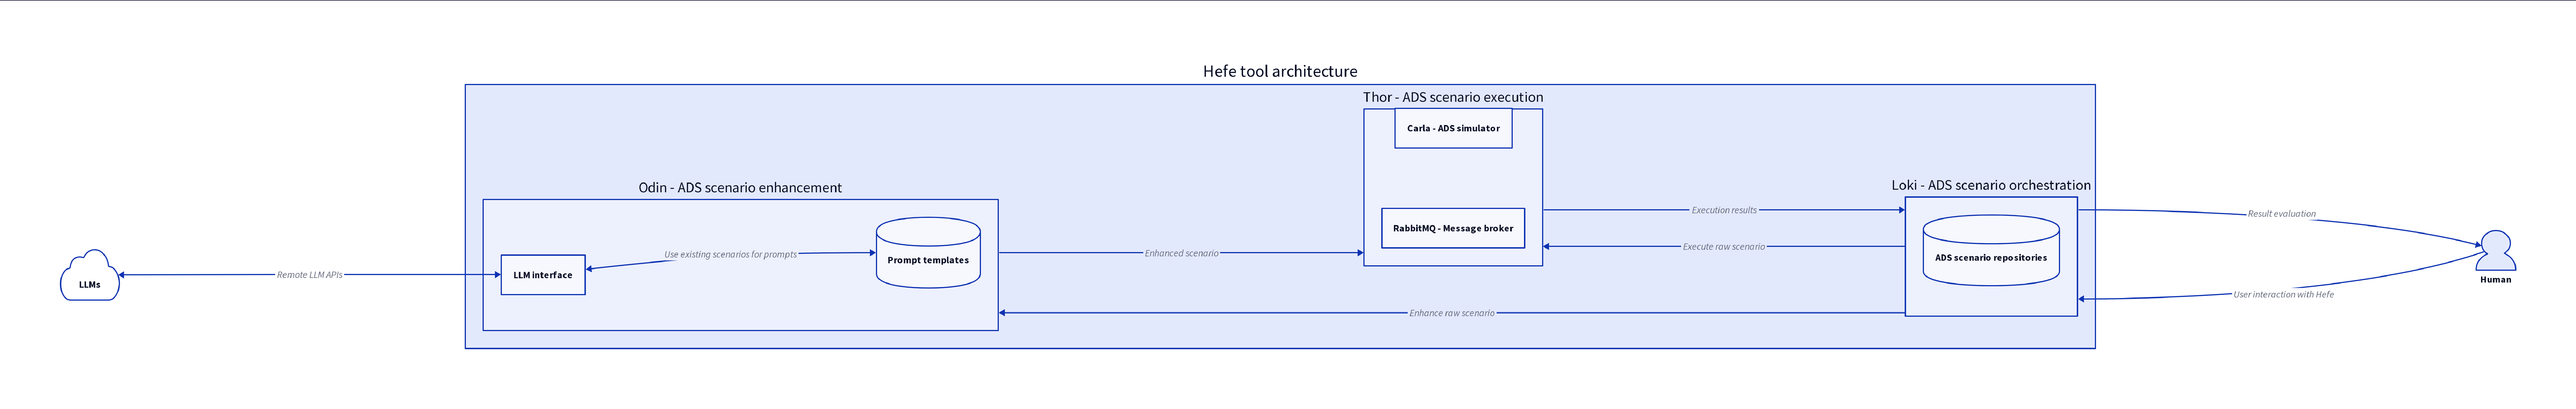
\includegraphics[width=\textwidth]{figures/d2-pdf/hefe.pdf}
    \caption{\hefe~pipeline architecture}\label{fig:hefeArch}
\end{figure}


Furthermore, as outlined in \citeauthor{LLM4AD}, \acrlongpl{llm} can be applied to several aspects
of \acrlong{ads}. We will however focus on the driveability of the scenarios, in line with the
\Nref{sec:problemDescription}.


% \section*{The applicability of \acrshortpl{llm} in \acrshort{ads} testing}
\section{Broad architectual overview}


\acrlong{ads} are typically modular, as we have seen in \Cref{sec:adsTestingComplexity}.
\acrshortpl{llm} are applicable to the different modules in different ways as we saw in
\Nref{chp:relatedWork}. In order to further our goal of decreasing the driveability of the
\acrshort{ads}, the module of our interest is the \emph{motion planner} -- the part of the
\acrshort{ads} responsible for determining where to go and what to do.

\begin{tcolorbox}[colback=gray!5!white,colframe=gray!75!black,title=User history
        of using \hefe]\label{user-history}
    I have a set of \acrfull{ads} test cases. I provide this set to \hefe. It will run the entire
    set, and generate a baseline of my \acrshort{ads} performance.

    \hefe~will then improve my test cases using \acrlongpl{llm} and run them again.

    Lastly \hefe~will report how the results differ from running the base and enhanced version of a
    test case.

    This will give me insight into what caused my \acrshort{ads} to fail so that I can look into the
    cause of the error state and uncover underlying faults in the \acrlong{ads}.

\end{tcolorbox}


\subsection{Implementation language}

The programming language \textsc{Python} is widely used for \acrfull{ads} simulation. It is a high
level language, allowing the user great flexibility and developer experience. For this reason, I
will implement \hefe~using Python.

Python can be optimized using \acrfull{jit} compilers such as Numba~\cite{numba}, which can speed up
our execution times. Libraries such as Joblib provide Python with plug-and-play
meomization, which will allow us to re-use values that have already been
computed, saving time and energy.


\subsection{Overview of the components of the \hefe~pipeline}\label{sec:hefeComponentOverview}

The pipeline architecture is visualised in \Nref{fig:hefeArch}. Here we
present the major components and their responsibilities.


\subsection*{Test case enhancement}

\subsubsection{Test case repositories}

We have seen in \Nref{chp:relatedWork} that there are existing repositories of
% TODO: Make more specific reference to what part of Related Work
\acrshort{ads} test cases. These will provide us with \begin{inparaenum}
    \item a baseline,
    and
    \item data onto which we can apply our \acrshort{llm} enhancements.
\end{inparaenum}

We do naturally have to walk before we can run. For this reason, the project will initially be
tested on simple test scenarios provided by people behind the Carla simulator. When we have verified
that the project is sufficiently working for its stated purpose, we can scale up the activities to
other datasets. Several are presented in \Nref{chp:relatedWork}. The concept of applying
\acrshortpl{llm} to \acrshort{ads} scenarios is quite universal in nature and is eligble for
application for virutally \emph{all} datasets.

\subsubsection{LLM enhancement}\label{sec:llmEnhancement}
% TODO: Dette må spisses mot driveability

The base test cases will individually be enhanced by prompting the
\acrshort{llm}. We will experiment with several \acrshortpl{llm}.

Note that we will not employ any traditional \acrfull{nlp} techniques related to e.g. tokenization
or input processing -- we will leave this up to the internal mechanisms of the \acrshortpl{llm}.

For performing the actual improvement, it is essential that we \begin{inparaenum}
    \item test several \acrshort{llm},
    \item give clear prompts
    % \info{I'm inclined to find some fitting prompts through trial and error, as such a I do not wish to describe them in detail at this time.}
    and
    \item verify that the returned test case adheres to the strictly necessary
    syntax rules. This last point is important due to our knowledge of
    \acrshortpl{llm} hallucinating (see \Nref{sec:llmProblems}).
    % TODO: More specific reference to Halucination intead of all LLm problems?
\end{inparaenum}

In order to facilitate testing various \acrlongpl{llm}, we should employ
\acrshort{llm} agnostic software as a translation layer. This will allow us to
write code for a common interface and test several \acrshortpl{llm} that may all
have different internal \acrfullpl{api} without having to modify our test code
for specific \acrshortpl{api}. This \begin{inparaenum}
    \item saves time
    and
    \item makes for more even test conditions \end{inparaenum}. Some pieces of software providing
this type of functionality include
\textsc{aisuite}\footnote{\url{https://github.com/andrewyng/aisuite}}, RamaLama from
RedHat\footnote{\url{https://github.com/containers/ramalama}}, and the MIT licensed
Ollama\footnote{\url{https://github.com/ollama/ollama}}, both supporting a plethora of
\acrlongpl{llm}.

% TODO: Burde fjerne disse random Github-prosjektene som ikke blir brukt i den faktiske implementasjonen?
\textsc{guidance}\footnote{\url{https://github.com/guidance-ai/guidance}} is a
framework for limiting the room in which \acrshortpl{llm} may operate, which
might be useful if we run into issues with excessive hallucination.


\subsubsection{Enhanced test case validation}

We must expect the \acrshort{llm} to hallucinate to some extent (\Cref{sec:llmHallucination}). We
therefore propose to verify the format of the enhanced file before running it.

As we saw in the section for \Nref{sec:adsScenarioFormats}, there exists several formats for
\acrshort{ads} scenarios. In order to verify that the syntax of our enhanced test
case is valid, we simply need to apply the syntax rules of our format.

The CommonRoad format is XML-based~\cite[720]{commonRoadOG} and as such we can
to some extent assess the degree of hallucination by parsing the XML structure.
Furthermore, it has an exhaustive Python library with several utilities\footnote{\url{https://pypi.org/user/commonroad/}}.

OpenSCENARIO exists both as XML and a domain-specific language (DSL). If we
utilise the XML version, we can apply the same methodology as for the CommonRoad
format. If using the DSL version, one way
the OpenSCENARIO format can be verified is by using free
online cloud services such as this offering from AVL
\footnote{\url{https://smc.app.avl.com/validation}}. We should however strive for
running a local verification service to \begin{inparaenum}
    \item save time and compute,
    and
    \item preserve data privacy.
\end{inparaenum}
Besides, it is generally a good idea to limit the number of external dependencies\footnote{Note for
    example how LGSVL\cite{lgsvl} was shut down, preventing projects such as DeepScenario of
    \citeauthor{DeepScenario} to be further developed on the original platform.}.

\subsection{Test case running and evaluation}

\subsubsection{Test case runner}

The system will automatically run all
our base test cases using an \acrshort{ads} simulator, and collect data points to get a baseline. It
will later also run the mutated \acrshort{llm}-enhanced versions of the base cases.

We have already ran the test cases in their base form. We will now run their
improved versions in order to compare them to see what effect the \acrshort{llm}
enhancement (see \Cref{sec:llmEnhancement}) has had.

For the reasons we have seen in~\Cref{sec:simulatorOverview}, we want to run our
test cases on Carla. It is the best offering as it is open source, under active
development and has a feature rich Python \acrshort{api}.

\subsubsection{Test case improvement evaluation}\label{sec:testCaseEval}

We saw in \Cref{sec:adsMetrics} that there are several metrics for assessing
\acrshort{ads}. We will use these metrics when evaluating our improvements.

\subsubsection{Test case result reporting}

We will compare the results from running
the baseline unmodified test case and comparing it with the results from
running the \acrshort{llm}-enhanced version and returning to the user. Ideally with
some automatic analysis of the results.

Having ran both the base test case and its enhanced counterpart, we have
results. The results will be stored in \acrfull{csv} files, allowing \begin{inparaenum}
    \item further analysis in Python/Jupyter,
    and
    \item easy translation to \LaTeX tables for the final report.
\end{inparaenum}

This is the final step of the envisioned pipeline. Where we have our result, and
need to analyse them.

This last step has great opportunities for being scoped up to a fully integrated
test suite which allows for both running test cases and analysing the results in
a \acrfull{gui}. But we should focus on the prior steps for now, only creating a
\acrshort{gui} if there is sufficient time towards the end of the project to
focus on such non-\acrshort{llm} related topics.

Initially, the results will consist of numerical comparison of the
\acrshort{csv}s with regard to the relevant metrics outlined in
\Nref{sec:testCaseEval}.

We need to define what requirement we will use for determining the \textit{result} of a test case
run. Without this, we cannot compare it to other test cases.

\section{Component details}

Having begotten a broad overview of the details of the \hefe~pipeline, let us now narrow our scope
and focus on the individual components.

% Alt under her er kopiert over fra det gamle "implementation details"-chpt.
% (Og så tilpasset litt, dekrementert heading levels osv )

The implementation is what facilitates doing the actual experiments. For the most part, it follows
what is outlined in the \Nref{sec:hefeComponentOverview}, with some minor practical differences.
What follows will analyze the impelementation of the components of the \hefe{} pipeline and explain
more closely in detail not only \emph{what} they do, as that is already covered in the solution
proposal, but \emph{how} they do it, with hands-on code examples.

% TODO: Burde avklare om den skal leve her "for alltid". Syns det kan gi emning
% å samle alle master ting i ett repo. Fortrinnsvis _dette_ (veldig meta å linke
% til seg selv i så fall hehe). Kan også være gunstig mtp å inkludere kode som appendix?
All code is available on the Github repo \href{https://github.com/orjahren/master-hefe}{\texttt{master-hefe}}.

\subsection{Carla interface and scenario utilities -- Thor}

The Thor module is responsible for all thigs related to the Carla \acrshort{ads}
simulator. It provides the client with several scenario-related utilities, and
is capable of executing the desired scenarios.


Certain of its utilities are simple tools for asserting the liveness of Carla,
such as the \texttt{get\_carla\_is\_up} function, shown in
listing~\ref{lst:odinCarlaHealthCheck}. This function will use the Caral
standard Python library and attempt to connect to the server on its default
port\footnote{I.e. \num{2000}, line \#4 in listing
    \ref{lst:odinCarlaHealthCheck}.}. Note that we refer to the host as simpyly
\texttt{carla} -- this is possible due to the entire project running
containerised with Docker Compose. Instead of refering to the speicifc IP
address of the Carla server (typically localhost, if not running it externally),
the Docker system will facilitate this name translation for us.

\lstinputlisting[caption={Exerpt from carla\_interface.py, demonstrating the implementation of a Carla health check.}, label={lst:odinCarlaHealthCheck}, language={Python}]{hefe-listings/carla_interface.py}

This is used both to assert the general liveness of the \hefe~pipeline, and to
verify that the simulator is available before performing experiments. It is
better to detect this illegal state \emph{before} running experiments rather
than during their execution.

Furthermore, it shall also be equipped with funcitonality for \emph{executing} \acrshort{ads}
scenarios on Carla. This is trivial when using Carla's existing Scenario Runner
module's funcitonality. As of now, this has not yet been implemented due to
greater challenges in the \acrshort{llm} module -- Odin.


% Rest API - running test cases - Thor
% “Fast API”, Python
% POST a test case to the API. It will be ran on the ‘server’
% RabbitMQ for listening for finished test cases? So that the client knows it can fetch the results?
% Will need UUID for test cases so the correct result can be fetched after it has been ran
% Need to store these somewhere. NoSQL database?
% This component should also accumulate results.
% Huge TODO: What metric are these results?
% Should be containerised (Docker/Podman)

\subsection{LLM interface and prompt applications -- Odin}\label{sec:odinImplementation}

% Rest API - performing LLM enhancement - Odin
% “Fast API”, Python
% Take a base test case as body
% Have some prompt repository
% Apply prompts with LLMs
% Must integrate with LLM. Either locally (Ollama) or remote (some API)
% Look into good LLM agnostic transition layer. E.g. Aisuite
% https://github.com/andrewyng/aisuite
% Should use same UUIDs as outlined above, but suffixed with e.g. “pure” and “tainted”
% Containerized. Docker compose?

The Odin module handles all things \acrshort{llm}. It provides a unified
\acrshort{api} for applying various prompts to scenarios and returning the
enhanced output resulting from having applied the prompt. We hve implemented
support for the \acrshortpl{llm} that are available on \begin{inparaenum}
    \item Ollama, and
    \item Gemini
\end{inparaenum}. This allows for testing with \acrshortpl{llm} such as
\begin{inparaenum}\setcounter{enumi}{2}
    \item Mistral \num{7.2}B, and
    \item gemini-2.5-flash
\end{inparaenum}.

\subsection*{LLM interface implementations}
\subsubsection{Gemini integration}

The Gemini integration is quite straightforward, relying on Google's own
\texttt{genai} Python module. Listing~\ref{lst:thorGeminiInterface} renders the
\emph{entire} interface, again highlighting how straightforward this really is.
The one piece of complexity to not is that it requires that the user provides
their own Gemini \acrshort{api} key and has this set as an environment variable
with the proper name. Without this being as it should, the script will crash, as
it would not possible for it to complete the desired \acrshort{llm} enhancement
regardless as long as the \acrshort{api} key is not present.

\lstinputlisting[caption={llm\_api\_interfaces/gemini\_interface.py, The implementation of a Gemini interface for executing prompts.}, label={lst:thorGeminiInterface}, language={Python}]{hefe-listings/gemini.py}

\subsubsection{Ollama integration}

The Ollama integration is a bit more cumbersome. This motly comes down to it not
using any exisitng library modules for this specific purpose, instead relying on
using the \texttt{json} and \texttt{requests} modules to implement the desired
funcitonality from scratch, making it so that we need to handle network IO and
marshalling the \acrfull{llm} response into a fitting return buffer.

Listing~\ref{lst:thorOllamaInterface} renders the
\emph{entire} interface. As we can see, it is not too bad allthough nowhere near
as clean as the Gemini implementation (\ref{lst:thorGeminiInterface}).

Its complexity arises principally from \num{2} major factors --
\begin{inparaenum}
    \item the already mentioned manual networking, and
    \item having to parse the streamed response
\end{inparaenum}
Furthermore, this code expects that the user already \emph{has} an Ollama
installation running on their host machine. The code provides no means of setup
for this -- that is an entirely external endeavour that is left up to the end user.

Similarly to how the Gemini implementation does it, this will crash if Ollama is
not funcitoning properly as it would not possible for it to complete the desired
\acrshort{llm} enhancement regardless if Ollama is unreachable.

\lstinputlisting[caption={llm\_api\_interfaces/ollama.py, The implementation of an Ollama interface for executing prompts.}, label={lst:thorOllamaInterface}, language={Python}]{hefe-listings/ollama.py}

\subsection*{Prompts and their associated code}

In this project, the prompts are the instruction to the \acrfull{llm} for
applying the enhancement to the scenario. Quite possibly the most critical piece
of code related to the experiments. They need to take the base scenario as an
input and integrate it into the \acrshort{llm} context, such that it knows what
it shall use as its base to apply enhancements that will decrease the
driveability. For this reason, it also provides certain scenario
utilities\footnote{That architectually might as well have been integrated in the
    Thor module\ldots}.

\subsubsection{Scenario utilities}

These are essentially quite trivial helpers. Lisitng \ref{lst:odinScenarioUtils}
renders the core functionality -- hopefully this is quite self-explaining.

\lstinputlisting[caption={scenario\_utils.py, The implementation of an various scenaro helper functions for executing prompts.}, label={lst:odinScenarioUtils}, language={Python}]{hefe-listings/scenario_utils.py}

\subsubsection{Prompts -- templating and usage}

% TODO: Finnes det noe bigbrain måte å slippe å manuelt måtte referere ti llinjenummer?
As mentioned, the prompts need to include the scenarios \emph{in} them, so that
they are accessible to the \acrshort{llm}. How this is done, is rendered in
listing~\ref{lst:odinPromptTestbed}. The most interesting aspect is how the
prompts are stored in the system as lambda functions. This makes it so that they
can take an argument that represents the scenario --
\texttt{python\_carla\_scenario\_raw}(line \#16) -- and simply \emph{execute} the
function to insert the scenario into the prompt (line \#42). This is then
inserted into the output prompt at the location located at line \#21 in the listing.

% TODO: Linjenummere må oppdateres
% TODO: Må legge til at man også kan passe inn scenario-navn og metrics

\lstinputlisting[caption={experiments/testbed/prompts.py, The implementation of a prompt testbed for executing prompts.}, label={lst:odinPromptTestbed}, language={Python}]{hefe-listings/testbed_prompts.py}

Lastly, note the comments in the top of the file, intended to give Github
Copilot increased understanding of the context, so that it can provide better
aid during programming.


\subsection{Execution tool / user oriented frontend -- Loki}

% Client - orchestrating the process - Loki
% Fetch available test cases from Thor? Select what/which are to be used
% Store results clientside? Separate database for this?

The final module of the \hefe~pipeline is Loki -- it is simply a tool intended
to be used by the user for operating the process. It \begin{inparaenum}
    \item  says what scenarios are available to it (i.e. those that are eligble for
    being enhanced), and
    \item allows the user to select a prompt and
    \item execute that prompt to the scenario of their choosing.
\end{inparaenum}

\lstinputlisting[caption={loki/main.py, The implementation of the Loki script.}, label={lst:lokiMainImplementation}, language={Python}]{hefe-listings/loki_main.py}

Listing~\ref{lst:lokiMainImplementation} renders the implementation of the
script. It relies on the Odin and Thor modules for all essential functionality,
which is in line with what is to be expected as this is simply a frontend client
to \emph{reach} them.

It is relies on the \texttt{requests} module for doing \acrfull{rpc} to the
other modules. There is also the outlines of a RabbitMQ implementation, which is
why \texttt{pika} is being imported. As of now, this is in non-functioning
alpha. Implementation of RabbitMQ message passing has not been prioritized as
there were, as mentioned, more important issues to focus on that would yield
better and more important results when resolved. This would maintain feature
parity with the \texttt{requests}-based approach.